%%%%%%%
% \newpage
\subsection{Bài tập tự luận}
% \BTTL
\setcounter{bt}{0}
%%==========Bài 1
\begin{bt}
	Cho $P(A)=0{,}2;P(B)=0{,}51;P(B\mid A)=0{,}8$. Tính $P(A\mid B)$.
	\loigiai{
		Ta có
		$P(AB)=P(A) \cdot P(B \mid A)=0{,}2\cdot 0{,}8=0{,}16$.\\
		$P(AB)=P(B) \cdot P(A \mid B) \Rightarrow P(A \mid B)=\dfrac{P(AB)}{P(B)}=\dfrac{0{,}16}{0{,}51}\approx 0{,}314$.
	}
\end{bt}

%%==========Bài 2
\begin{bt}
	Cho hai biến độc lập $A,B$ với $\mathrm{P}(A)=0{,}8$, $\mathrm{P}(B)=0{,}25$. Tính $\mathrm{P}(A\mid B)$.
	\loigiai{
		Vì $A$ và $B$ là hai biến cố độc lập, do đó
		\[\mathrm{P}(A\mid B)=\dfrac{\mathrm{P}(A\cap B)}{\mathrm{P}(B)}=\dfrac{\mathrm{P}(A)\cdot\mathrm{P}(B)}{\mathrm{P}(B)}=\mathrm{P}(A)=0{,}8.\]	
	}
\end{bt}
%%==========Bài 3
\begin{bt}
	Cho hai biến cố $A$, $B$ có $\mathrm{P}(A)=0{,}6;\mathrm{P}(B)=0{,}8;\mathrm{P}(A\cap B)=0{,}4$. Tính các xác suất sau:
	\begin{listEX}[2]
		\item $\mathrm{P}(B\mid A);\mathrm{P}(\overline{B}\mid A)$.
		\item $\mathrm{P}(A \cap \overline{B})$.
	\end{listEX}
	\loigiai{
		\begin{enumerate}
			\item $\mathrm{P}(B\mid A)=\dfrac{\mathrm{P}(A \cap B)}{\mathrm{P}(A)}=\dfrac{0{,}4}{0{,}6}=\dfrac{2}{3} 
			\Rightarrow \mathrm{P}(\overline{B}\mid A)=1-\mathrm{P}(B\mid A) = 1 -\dfrac{2}{3}=\dfrac{1}{3}$.
			\item Ta có 
			\begin{eqnarray*}
				\mathrm{P}(A \cap \overline{B}) &=& \mathrm{P}\left(\overline{B}\mid A\right)\cdot \mathrm{P} (A)=\dfrac{1}{3}\cdot 0{,}6=0{,}2.
			\end{eqnarray*}
	\end{enumerate}}
\end{bt}
%%==========Bài 5
\begin{bt}%[2D5H1-2]
	Cho hai biến cố $A$ và $B$ có $P(A)=0{.}4; P(B)=0{.}8$ và $P(A|B)=0{.}5$. Tính $P(A\overline{B})$ và $P(A|B)$.
	\loigiai{
		Ta có $P(A\overline{B})=P(A|\overline{B})\cdot P(\overline{B})=0{.}5\cdot 0{.}2=0{.}1$.\\
		Vì $AB$ và $A\overline{B}$ là hai biến cố xung khắc và $AB\cup A\overline{B}=A$ nên theo tính chất của xác suất, ta có\\ $P(AB)=P(A)-P(A\overline{B})=0{.}4-0{.}1=0{.}3$.\\
		Khi đó: $P(A|B)=\dfrac{P(AB)}{P(B)}=\dfrac{0{.}3}{0{.}8}=0{.}375$.
	}
\end{bt}
%%==========Bài 4
\begin{bt}%[2D5B1-2]
	Một thư viện có $35\%$ tổng số sách là sách khoa học, $14\%$ tổng số sách là sách khoa học tự nhiên. Chọn ngẫu nhiên một quyển sách của thư viện. Tính xác suất để quyển sách được chọn là sách khoa học tự nhiên, biết rằng đó là quyển sách về khoa học.
	\loigiai
	{Gọi $A$ là biến cố \lq\lq  Sách được chọn là sách khoa học tự nhiên\rq\rq.\\
	Gọi $B$ là biến cố \lq\lq  Sách được chọn là sách khoa học\rq\rq.\\
	Do có $35\%$ tổng số sách là sách khoa học nên $P(B)=0{.}35$.\\
	Do có $14\%$ tổng số sách là sách khoa học tự nhiên nên $P(AB)=0{.}14$.\\
	Vậy $P(A|B)=\dfrac{P(AB)}{P(B)}=\dfrac{0{.}14}{0{.}35}=0{.}4$.
	}
\end{bt}


%%==========Bài 7
\begin{bt}
	Một hộp kín đựng 20 tấm thẻ giống hệt nhau đánh số từ 1 đến 20. Một người rút ngẫu nhiên ra một tấm thẻ từ trong hộp. Người đó được thông báo rằng thẻ rút ra mang số chẵn. Tính xác suất để người đó rút được thẻ số 10.
	\loigiai{
	Gọi $A$ là biến cố: ``Người đó rút được thẻ số 10''.\\
	Gọi $B$ là biến cố: ``Người đó rút được thẻ mang số chẵn''.\\
	Không gian mẫu mà 20 tấm thẻ đánh số từ 1 đến 20 $\Rightarrow$ $n(\Omega)=20$.\\
	Ta cần tính $P\left(A\mid B\right)$.\\
	Ta có, từ 1 đến 20 có 10 số chẵn nên $n(B)=10$.\\
	Vậy $P(B)=\dfrac{n(B)}{n(\Omega)}=\dfrac{10}{20}=\dfrac{1}{2}$.\\
	Trong số 10 số chẵn có một số 10 nên $n(AB)=1$.\\
	Vậy $P(AB)=\dfrac{n(AB)}{n(\Omega)}=\dfrac{1}{20}$.\\
	Do đó $P(A\mid B)=\dfrac{P(AB)}{P(B)}=\dfrac{1}{10}\approx 0{,}1$.
	}
\end{bt}

%%==========Bài 8
\begin{bt}
	Gieo hai con xúc xắc cân đối, đồng chất. Tính xác suất để:
	\begin{enumerate}[a)]
	\item Tổng số chấm xuất hiện trên hai con xúc xắc bằng 7 nếu biết rằng ít nhất có một con xúc xắc xuất hiện mặt 5 chấm;
	\item Có ít nhất có một con xúc xắc xuất hiện mặt 5 chấm nếu biết rằng tổng số chấm xuất hiện trên hai con xúc xắc bằng 7. 
	\end{enumerate}
	\loigiai{
	\begin{enumerate}[a)]
	\item Không gian mẫu $n(\Omega)=6\cdot 6=36$.\\
	Gọi $A$ là biến cố: ``Tổng số chấm xuất hiện trên hai con xúc xắc bằng 7''.\\
	Gọi $B$ là biến cố: ``Có ít nhất một con xúc xắc xuất hiện mặt 5 chấm''.\\
	Ta có $n(B)=6+6+1=13$ ứng với các trường hợp $(5;x)$; $(x;5)$; $(5;5)$.\\
	Vậy $P(B)=\dfrac{n(B)}{n(\Omega)}=\dfrac{13}{36}$.\\
	Ta có tổng số chấm xuất hiện trên hai con xúc xắc bằng 7 trong đó có ít nhất một con xúc xắc xuất hiện mặt 5 chấm ứng với các trường hợp $(5;2)$ và $(2;5)$. \\
	Suy ra $n(AB)=2$.\\
	Vậy $P(AB)=\dfrac{n(AB)}{n(\Omega)}=\dfrac{2}{36}=\dfrac{1}{18}$.\\
	Do đó 
	$P(A\mid B)=\dfrac{P(AB)}{P(B)}=\dfrac{2}{13}$.
	\item Ta tính $P(B\mid A)$.\\
	Biến cố tổng hai mặt là $7: A=\{(1;6);(2;5);(3;4);(4;3);(5;2);(6;1)\}$ nên $n(A)=6$.\\
	Vậy $P(A)=\dfrac{n(A)}{n(\Omega)}=\dfrac{6}{36}$.\\
	Ta có $P(BA)=P(AB)=\dfrac{1}{18}$.\\
	Do đó 
	$P(B\mid A)=\dfrac{P(BA)}{P(A)}=\dfrac{2}{6}=\dfrac{1}{3}$.
	\end{enumerate}
	}
\end{bt}
%%==========Bài 9
\begin{bt}
	Gieo hai con xúc xắc cân đối, đồng chất. Tính xác suất để tổng số chấm xuất hiện trên hai con xúc xắc đó không nhỏ hơn 10 nếu biết rằng có ít nhất một con xúc xắc xuất hiện mặt 5 chấm.
	\loigiai{
	Không gian mẫu $n(\Omega)=6\cdot 6=36$.\\
	Gọi $A$ là biến cố: ``Tổng số chấm xuất hiện trên hai con xúc xắc không nhỏ hơn 10''.\\
	Gọi $B$ là biến cố: ``Có ít nhất một con xúc xắc xuất hiện mặt 5 chấm''.\\
	Ta có $n(B)=6+6+1=13$ ứng với các trường hợp $(5;x)$; $(x;5)$; $(5;5)$.\\
	Vậy $P(B)=\dfrac{n(B)}{n(\Omega)}=\dfrac{13}{36}$.\\
	Ta có tổng số chấm xuất hiện trên hai con xúc xắc không nhỏ hơn 10 trong đó có ít nhất một con xúc xắc xuất hiện mặt 5 chấm ứng với các trường hợp $(5;5);(5;6);(6;5)$.\\
	Suy ra $n(AB)=3$.\\
	Vậy $P(AB)=\dfrac{n(AB)}{n(\Omega)}=\dfrac{3}{36}=\dfrac{1}{12}$.\\
	Do đó 
	$P(A\mid B)=\dfrac{P(AB)}{P(B)}=\dfrac{3}{13}$.
	}
\end{bt}



%%==========Bài 12
\begin{bt}
	Một hộp có $3$ quả bóng màu xanh, $4$ quả bóng màu đỏ; các quả bóng có kích thước và khối lượng như nhau. Lấy bóng ngẫu nhiên hai lần liên tiếp, trong đó mỗi lần lấy ngẫu nhiên một quả bóng trong hộp, ghi lại màu của quả bóng lấy ra và bỏ lại quả bóng đó vào hộp. Xét các biến cố:
	\begin{enumerate}
	\item $A$ \lq\lq  \,Quả bóng màu xanh được lấy ra ở lần thứ nhất\rq\rq;
	\item $B$ \lq\lq  \,Quả bóng màu đỏ được lấy ra ở lần thứ hai \rq\rq.
	\end{enumerate}
	Chứng minh rằng $A$, $B$ là hai biến cố độc lập.
	\loigiai{
	Gọi $A_i$ là biến cố \lq\lq  Lần thứ $i$ lấy được bóng màu xanh\rq\rq:\\
	$A=A_1A_2 \cup \overline{A_1}~\overline{A_2} \Rightarrow P\left(A\right)=\dfrac{3}{7}\cdot\dfrac{3}{7}+\dfrac{3}{7}\cdot\dfrac{4}{7}=\dfrac{3}{7}$.\\
	Gọi $B_i$ là biến cố \lq\lq  Lần thứ $i$ lấy được bóng màu đỏ\rq\rq:\\
	$B=B_1B_2 \cup \overline{B_1}B_2 \Rightarrow P\left(B\right)=\dfrac{4}{7}\cdot\dfrac{4}{7}+\dfrac{4}{7}\cdot\dfrac{3}{7}=\dfrac{4}{7}$.\\
	Ta có, $\mathrm{P}(A\mid B)=\dfrac{n\left(A \cap B\right)}{n\left(B\right)}=\dfrac{4\cdot 3}{7\cdot 4}=\dfrac{3}{7}=P\left(A\right) \Rightarrow A, B$ là hai biến cố độc lập.}
\end{bt}
%%==========Bài 13
\begin{bt}
	Cho hai con xúc xắc cân đối và đồng chất. Gieo lần lượt từng xúc xắc trong hai xúc xắc đó. Tính xác suất để tổng số chấm xuất hiện trên hai xúc xắc bằng $6$, biết rằng xúc xắc thứ nhất xuất hiện mặt $4$ chấm.
	\loigiai{
	Gọi $A$ là biến cố \lq\lq  xúc xắc thứ nhất xuất hiện mặt $4$ chấm\rq\rq ~và $B$ là biến cố \lq\lq  tổng số chấm xuất hiện trên hai xúc xắc bằng $6$\rq\rq.\\
	Xác suất của $A$ là $\mathrm{P}(A)$ là xác suất để xúc xắc thứ nhất xuất hiện mặt $4$ chấm. Vì xúc xắc cân đối và đồng chất, nên \[\mathrm{P}(A)=\dfrac{1}{6}.\]
	Xác suất của $B$ khi biết $A$ đã xảy ra là $\mathrm{P}(B \mid A)$. Trong trường hợp này, để tổng số chấm là $6$, xúc xắc thứ hai phải xuất hiện mặt $2$ chấm. Do đó, $\mathrm{P}(B \mid A)=\dfrac{1}{6}$.\\
	Vậy, theo quy tắc xác suất điều kiện, ta có:\\
	$$\mathrm{P}(B \mid A)=\dfrac{\mathrm{P}(A \cap B)}{\mathrm{P}(A)} \Rightarrow \mathrm{P}(A \cap B)=\mathrm{P}(B \mid A)\cdot \mathrm{P}(A)=\dfrac{1}{6}\cdot \dfrac{1}{6}=\dfrac{1}{36}.$$
	}
\end{bt}
%%==========Bài 14
\begin{bt}
	Một doanh nghiệp trước khi xuất khẩu áo sơ mi phải qua hai lần kiểm tra chất lượng sản phẩm, nếu cả hai lần đều đạt thì chiếc áo đó mới đủ tiêu chuẩn xuất khẩu. Biết rằng bình quân $98\%$ sản phẩm làm ra qua được lần kiểm tra thứ nhất và $95\%$ sản phẩm qua được lần kiểm tra thứ nhất sẽ tiếp tục qua được lần kiểm tra thứ hai. Tính xác suất để một chiếc áo sơ mi đủ tiêu chuẩn xuất khẩu.
	\loigiai{
	$A$ là biến cố \lq\lq  sản phẩm qua được lần kiểm tra thứ nhất\rq\rq.\\
	$B$ là biến cố \lq\lq  sản phẩm qua được lần kiểm tra thứ hai\rq\rq.\\
	Bài toán yêu cầu tính xác suất của biến cố $A\cap B$, tức là sản phẩm vừa qua được lần kiểm tra thứ nhất, và sau đó qua được lần kiểm tra thứ hai.\\
	Xác suất của $A$ là $\mathrm{P}(A)=0{,}98$.\\
	Xác suất của $B$ khi đã qua được $A$ là $\mathrm{P}(B \mid A)=0{,}95$.\\
	Áp dụng công thức xác suất có điều kiện, ta có:
	$$\mathrm{P}(A \cap B)=\mathrm{P}(A)\cdot \mathrm{P}(B \mid A)=0{,}98\cdot 0{,}95=0{,}931.$$
	Vậy, xác suất để một chiếc áo sơ mi đủ tiêu chuẩn xuất khẩu là $93{,}1\%$
	}
\end{bt}
%%==========Bài 17
\begin{bt}
	Một nhóm $50$ học sinh có $23$ bạn biết chơi cầu lông mà không biết chơi bóng đá và $21$ bạn biết chơi bóng đá mà không biết chơi cầu lông. Biết rằng mỗi học sinh trong nhóm này biết chơi bóng đá hoặc cầu lông. Chọn ngẫu nhiên một học sinh trong nhóm. Tính xác suất học sinh này biết chơi bóng đá, biết rằng bạn ấy biết chơi cầu lông. 
	\loigiai{
		Gọi $A$ là biến cố "Học sinh được chọn biết chơi bóng đá"; $B$ là biến cố "Học sinh được chọn biết chơi cầu lông".\\
		Ta có $n\left(A\cap B\right)=50-(23+21)=6$ và $n(B)=23+6=29$. Do đó 
		$\mathrm{P}(A|B)=\dfrac{n\left(A\cap B\right)}{n(B)}=\dfrac{6}{29}$.
	}
\end{bt}
%%==========Bài 16
\begin{bt}
	Có $2$ linh kiện điện tử, xác suất để mỗi linh kiện hỏng trong một thời điểm bất kì lần lượt là: $0{,}01$; $0{,}02$. Hai linh kiện đó được lắp vào một mạch điện theo sơ đồ ở \textit{Hình a, b}. Trong mỗi trường hợp, hãy tính xác suất để trong mạch điện có dòng điện chạy qua
	\begin{center}
	\tikzset{noratorW/.style={voosource,
	bipoles/oosource/circlesize=0.5,
	bipoles/oosource/circleoffset=0.5},
	nullatorW/.style={esource, sources/scale=0.8}}
	\begin{tikzpicture}
	\draw (0,0) to[nullatorW] ++(2,0) to[nullatorW] ++(2, 0)--(4,-2)to[battery1](0,-2)--(0,0);
	\draw (2,-2.5) node[below] {\textit{a)}};
	\end{tikzpicture}
	\quad
	\begin{tikzpicture}
	\draw (0,0) to[battery1](4,0)--(4,-2)to[nullatorW](0,-2)--(0,0);
	\draw (4,-1) to[nullatorW](0,-1);
	\draw (2,-2.5) node[below] {\textit{b)}};
	\end{tikzpicture}
	\end{center}
	\loigiai{
	Gọi
	\begin{itemize}
	\item	$A$: \lq\lq  Linh kiện thứ nhất không hỏng\rq\rq .
	\item 	$B$: \lq\lq  Linh kiện thứ hai không hỏng\rq\rq.
	\end{itemize}
	\begin{enumerate}
	\item \textbf{Hai linh kiện mắc nối tiếp.}\\
	Xác suất để cả hai linh kiện đều không hỏng là:
	$$\mathrm{P}(A \cap B)=\mathrm{P}(A)\cdot \mathrm{P}(B \mid A)$$
	Ta có\\
	$\mathrm{P}(A)=1-P(\overline{A})=1-0{,}01=0{,}99$.\\
	$\mathrm{P}(B \mid A)=1-P(\overline{B}\mid A)=1-0{,}02=0{,}98$.\\
	$\Rightarrow \mathrm{P}(A \cap B)=\mathrm{P}(A)\cdot \mathrm{P}(B \mid A)=0{,}99\cdot0{,}98=0{,}9702$.
	\item \textbf{Hai linh kiện mắc song song.}\\
	Xác suất để ít nhất một linh kiện không hỏng là:
	$$\mathrm{P}	(A \cup B)=\mathrm{P}(A)+\mathrm{P}(B)-\mathrm{P}(A \cap B) = 0{,}99+0{,}98-0{,}9702=0{,}9998.$$
	\end{enumerate}
	}
\end{bt}
%%==========Bài 6
\begin{bt}%[2D5V1-3]
	Mỗi bạn học sinh trong lớp của Minh lựa chọn một trong hai ngoại ngữ là tiếng Anh hoặc tiếng Nhật. Xác suất chọn tiếng Anh của mỗi bạn học sinh nữ là $0{.}6$ và của mỗi bạn học sinh nam là $0{.}7$. Lớp của Minh có $25$ bạn nữ và $20$ bạn nam. Chọn ra ngẫu nhiên một bạn trong lớp.
	Sử dụng sơ đồ hình cây, tính xác suất của các biến cố 
	A:\lq\lq  Bạn được chọn là nam và học tiếng Nhật\rq\rq.\\
	B:\lq\lq  Bạn được chọn là nữ và học tiếng Anh\rq\rq .
	\loigiai{ 
		Gọi $A$ là biến cố \lq\lq  Bạn được chọn là nữ\rq\rq và $B$ là biến cố: \lq\lq  Bạn được chọn học tiếng Anh\rq\rq. \\
		Ta có
		$
		P(Y|X)=0{.}6; P(Y \mid \bar{X})=0{.}7 ; P(X)=\dfrac{5}{9}
		$.\\
		Do đó $P(\bar{X})=1-P(X)=\dfrac{4}{9} ; P(\bar{Y} |X)=1-P(Y|X)=0{.}4; \\P(\bar{Y} \mid \bar{X})=1-P(Y \mid \bar{X})=0{.}3$.\\
		Ta có sơ đồ hình cây như sau
		\begin{center}
			\begin{tikzpicture}[yscale=0.9]
				\def\gocm{20}
				\def\gocn{10}
				\def\r{4}
				\tikzset{s/.style={outer sep=0.5 mm,draw=magenta,rectangle,minimum width=2.75cm,rounded corners=1mm}}
				\path(0,0)node(O){}++(\gocm:\r)node[s](A1){X}++(\gocn:\r)node[s](A2){$Y$};
				\path(A1)++({-\gocn}:\r)node[s](a2){$\bar{Y}$};
				\path(O)++(-\gocm:\r)node[s](B1){$\bar{X}$}++(\gocn:\r)node[s](B2){$Y$};
				\path(B1)++({-\gocn}:\r)node[s](b2){$\bar{Y}$};
				\foreach \x/\y in {
					O/A1,A1/A2,
					O/B1,B1/B2,
					A1/a2,
					B1/b2}
				\draw[-stealth](\x.east)--(\y.west);
				\path(O)--(A1.west)node[pos=0.5,above]{$\dfrac{5}{9}$}(O)--(B1.west)node[pos=0.5,below]{$\dfrac{4}{9}$}(B1.east)--(B2.west)node[pos=0.5,above,sloped]{$0{.}7$}(A1.east)--(A2.west)node[pos=0.5,above,sloped]{$0{.}6$}
				(A1.east)--(a2.west)node[pos=0.5,below,sloped]{$0{.}4$}
				(B1.east)--(b2.west)node[pos=0.5,below,sloped]{$0{.}3$};
			\end{tikzpicture}
		\end{center}
		Do $A=\overline{X}\cdot\overline{Y}$ nên $P(\overline{X}\cdot\overline{Y})=\dfrac{4}{9}\cdot 0{.}3=\dfrac{2}{15}$.\\
		Do $B=XY$ nên $P(XY)=\dfrac{5}{9}\cdot 0{.}6=\dfrac{1}{3}$.\\
	}
\end{bt}
%%==========Bài 10
\begin{bt}
	Bạn An phải thực hiện hai thí nghiệm liên tiếp. Thí nghiệm thứ nhất có xác suất thành công là 0,7. Nếu thí nghiệm thứ nhất thành công thì xác suất thành công của thí nghiệm thứ hai là 0,9. Nếu thí nghiệm thứ nhất không thành công thì xác suất thành công của thí nghiệm thứ hai chỉ là 0,4. Tính xác suất để:
	\begin{enumerate}[a)]
		\item Cả hai thí nghiệm đều thành công;
		\item Cả hai thí nghiệm đều không thành công;
		\item Thí nghiệm thứ nhất thành công và thí nghiệm thứ hai không thành công. 
	\end{enumerate}
	\loigiai{
		Ta có sơ đồ hình cây
		\begin{center}
			\begin{tikzpicture}[line join = round,line cap = round, >=stealth, thick, font = \small, yscale = 0.85]
				%	\draw[gray!50,xstep = 1, ystep = 1] (-5,-5) grid (5,5);
				\path
				(0,0) coordinate (0) node[above=3mm] {TN}
				+(-2,-3) coordinate (11) node[left=3mm] {TB1}
				+(2,-3) coordinate (12) node[right=3mm] {TC1}
				(11)+(-1,-3) coordinate (21) node[below=3mm] {TB2} node[below=9mm] {TB1-TB2}
				+(1,-3) coordinate (22) node[below=3mm] {TC2} node[below=9mm] {TB1-TC2}
				(12)+(-1,-3) coordinate (23) node[below=3mm] {TB2} node[below=9mm] {TC1-TB2}
				+(1,-3) coordinate (24) node[below=3mm] {TC2} node[below=9mm] {TC1-TC2}
				(0)--(11) node[midway,left=3mm] {$\dfrac{3}{10}$}
				(0)--(12) node[midway,right=3mm] {$\dfrac{7}{10}$}
				(11)--(21) node[midway,left=2mm] {$\dfrac{6}{10}$}
				(11)--(22) node[midway,right=2mm] {$\dfrac{4}{10}$}
				(12)--(23) node[midway,left=2mm] {$\dfrac{1}{10}$}
				(12)--(24) node[midway,right=2mm] {$\dfrac{9}{10}$}
				;
				\draw (11)--(0)--(12)
				(21)--(11)--(22)
				(23)--(12)--(24)
				;
				\node[circle, line width = .2 mm, draw = black, text = black, fill = yellow!60, anchor = center, outer sep = 0pt, minimum size = .2cm] (c) at (0) {};
				\node[circle, line width = .2 mm, draw = black, text = black, fill = black, anchor = center, outer sep = 0pt, minimum size = .2cm] (c) at (11) {};
				\node[circle, line width = .2 mm, draw = black, text = black, fill = cyan, anchor = center, outer sep = 0pt, minimum size = .2cm] (c) at (12) {};
				\node[circle, line width = .2 mm, draw = black, text = black, fill = black, anchor = center, outer sep = 0pt, minimum size = .2cm] (c) at (21) {};
				\node[circle, line width = .2 mm, draw = black, text = black, fill = cyan, anchor = center, outer sep = 0pt, minimum size = .2cm] (c) at (22) {};
				\node[circle, line width = .2 mm, draw = black, text = black, fill = black, anchor = center, outer sep = 0pt, minimum size = .2cm] (c) at (23) {};
				\node[circle, line width = .2 mm, draw = black, text = black, fill = cyan, anchor = center, outer sep = 0pt, minimum size = .2cm] (c) at (24) {};
			\end{tikzpicture}
		\end{center}
		\begin{enumerate}[a)]
			\item Xác suất cả hai thí nghiệm đều thành công là $$\dfrac{7}{10}\cdot \dfrac{9}{10}=\dfrac{63}{100}.$$
			\item Xác suất cả hai thí nghiệm đều không thành công là $$\dfrac{3}{10}\cdot \dfrac{6}{10}=\dfrac{18}{100}.$$
			\item Xác suất thí nghiệm thứ nhất thành công và thí nghiệm thứ hai không thành công là $$\dfrac{7}{10}\cdot \dfrac{1}{10}=\dfrac{7}{100}.$$
		\end{enumerate}
	}
\end{bt}
%%==========Bài 11
\begin{bt}
	Trong một túi có một số chiếc kẹo cùng loại, chỉ khác màu, trong đó có 6 cái kẹo màu cam, còn lại là kẹo màu vàng. Hà lấy ngẫu nhiên một cái kẹo từ trong túi, không trả lại.
	Sau đó Hà lại lấy ngẫu nhiên thêm một cái kẹo khác từ trong túi. Biết rằng xác suất Hà lấy được cả hai cái kẹo màu cam là $\dfrac{1}{3}$. Hỏi ban đầu trong túi có bao nhiêu cái kẹo?
	\loigiai{
		Gọi số kẹo là $x~(x>6)$.\\
		Số kẹo màu vàng là $x-6$.\\
		Khi Hà lấy được chiếc kẹo màu cam thì số kẹo trong túi là $x-1$ và số kẹo cam còn lại trong túi là 5 cái.\\
		Ta có sơ đồ cây
		\begin{center}
			\begin{tikzpicture}[line join = round,line cap = round, >=stealth, thick, font = \small, yscale = 0.85]
				%	\draw[gray!50,xstep = 1, ystep = 1] (-5,-5) grid (5,5);
				\path
				(0,0) coordinate (0) node[above=3mm] {Túi kẹo}
				+(-2,-3) coordinate (11) node[left=3mm] {C}
				+(2,-3) coordinate (12) node[right=3mm] {V}
				(11)+(-1,-3) coordinate (21) node[below=3mm] {C} node[below=9mm] {CC}
				+(1,-3) coordinate (22) node[below=3mm] {V} node[below=9mm] {CV}
				(12)+(-1,-3) coordinate (23) node[below=3mm] {C} node[below=9mm] {VC}
				+(1,-3) coordinate (24) node[below=3mm] {V} node[below=9mm] {VV}
				(0)--(11) node[midway,left=3mm] {$\dfrac{6}{x}$}
				(0)--(12) node[midway,right=3mm] {$\dfrac{x-6}{x}$}
				(11)--(21) node[midway,left=2mm] {$\dfrac{5}{x-1}$}
				(11)--(22) node[midway,right=2mm] {$\dfrac{x-6}{x-1}$}
				(12)--(23) node[midway,left=2mm] {$\dfrac{6}{x-1}$}
				(12)--(24) node[midway,right=2mm] {$\dfrac{x-7}{x-1}$}
				;
				\draw (11)--(0)--(12)
				(21)--(11)--(22)
				(23)--(12)--(24)
				;
				\node[circle, line width = .2 mm, draw = black, text = black, fill = yellow!50!orange, anchor = center, outer sep = 0pt, minimum size = .2cm] (c) at (0) {};
				\node[circle, line width = .2 mm, draw = black, text = black, fill=orange, anchor = center, outer sep = 0pt, minimum size = .2cm] (c) at (11) {};
				\node[circle, line width = .2 mm, draw = black, text = black, fill = yellow, anchor = center, outer sep = 0pt, minimum size = .2cm] (c) at (12) {};
				\node[circle, line width = .2 mm, draw = black, text = black, fill = orange, anchor = center, outer sep = 0pt, minimum size = .2cm] (c) at (21) {};
				\node[circle, line width = .2 mm, draw = black, text = black, fill = yellow, anchor = center, outer sep = 0pt, minimum size = .2cm] (c) at (22) {};
				\node[circle, line width = .2 mm, draw = black, text = black, fill = orange, anchor = center, outer sep = 0pt, minimum size = .2cm] (c) at (23) {};
				\node[circle, line width = .2 mm, draw = black, text = black, fill = yellow, anchor = center, outer sep = 0pt, minimum size = .2cm] (c) at (24) {};
			\end{tikzpicture}
		\end{center}
		Xác suất để Hà lấy được cả hai cái kẹo màu cam là
		$$
		\dfrac{6}{x}\cdot \dfrac{5}{x-1}=\dfrac{1}{3} \Rightarrow x^2-x-90=0 \Rightarrow \hoac{&x=-9~\text{(loại)}\\&x=10~\text{thỏa mãn}.}
		$$
		Vậy ban đầu trong túi có 10 cái kẹo.
	}
\end{bt}











%%==========Bài 15
\begin{bt}
	Trên giá sách có $10$ quyển sách Khoa học và $15$ quyển sách Nghệ thuật. Có $9$ quyển sách viết bằng tiếng Anh, trong đó $3$ quyển sách Khoa học có $6$ quyển sách Nghệ thuật, các quyển sách còn lại viết bằng tiếng Việt. Lấy ngẫu nhiên một quyển sách. Dùng sơ đồ hình cây, tính xác suất để quyển sách được lấy ra là sách viết bằng tiếng Việt, biết rằng quyển sách đó là sách Khoa học.
	\loigiai{
		Gọi các biến cố:\\
		$A$: \lq\lq  Sách lấy ra là sách tiếng Việt\rq\rq.\\
		$B$: \lq\lq  Sách lấy ra là sách khoa học\rq\rq.\\
		Khi đó, xác suất để cuốn sách được lấy ra là tiếng Việt, biết rằng cuốn sách đó là sách khoa học là $\mathrm{P}\left(A\mid B\right)$.
		Ta có sơ đồ cây
		\begin{center}
			\begin{tikzpicture}[scale=.2,>=stealth,every node/.style={shape=rectangle,draw,rounded corners, color=blue, fill=blue!10}]
			%-------------
			\tikzstyle{block} = [rectangle, draw, fill=blue!10, rounded corners, text centered, text width = 10em, minimum height = 2em]
			%-------------
			\node (c1) {Cuốn sách được lấy};
			\node (c2) [block, above right = 4cm of c1]{$B\colon$ \,\lq\lq  Sách lấy ra là sách khoa học \rq\rq};
			\node at (7,7.5){$\mathrm{P}(B)=2/5$};
			\node at (7,-7.5){$\mathrm{P}(\overline{B})=3/5$};
			\node (c3) [block, below right= 4cm of c1]{$\overline{B}\colon$\,\lq\lq  Sách lấy ra là sách nghệ thuật \rq\rq};
			\node at (37.8,25){$\mathrm{P}(A\mid B)=7/10$};
			\node (c4) [above right = 2cm of c2]{$A\colon $\,\lq\lq  Sách lấy ra là sách tiếng Việt \rq\rq };
			\node (c5) [below right = 2cm of c2]{$\overline{A}\colon $\,\lq\lq  Sách lấy ra là sách tiếng Anh \rq\rq};
			\node at (39,9.5){$\mathrm{P}(\overline{A}\mid B)=3/10$};
			\node (c6) [block, above right =2cm of c3]{$A\colon $\,\lq\lq  Sách lấy ra là sách tiếng Việt \rq\rq };
			\node at (39,-8.5){$\mathrm{P}(A\mid \overline{B})=3/5$};
			\node (c7) [block, below right = 2cm of c3]{$\overline{A}\colon $\,\lq\lq  Sách lấy ra là sách tiếng Anh \rq\rq};
			\node at (39,-27.8){$\mathrm{P}(\overline{A}\mid \overline{B})=2/5$};
			%--------------
			\draw[->] (c1.east) -- (c2.west);
			\draw[->] (c1.east) -- (c3.west);
			\draw[->] (c2.east) -- (c4.west);
			\draw[->] (c2.east) -- (c5.west);
			\draw[->] (c3.east) -- (c6.west);
			\draw[->] (c3.east) -- (c7.west);
		\end{tikzpicture}
		\end{center}
		Từ đó ta có xác suất để cuốn sách lấy ra là tiếng Việt, biết rằng cuốn sách đó là sách khoa học là $\mathrm{P}(A\mid B)=\dfrac{7}{10}=0{,}7$.
	}
\end{bt}